%==============================================================================
% Chapitre 51 - Les projectiles militaires
%==============================================================================

\section{Introduction}

Les besoins militaires ont conduit au développement d'un grand nombre de
projectiles spécialisés.

Bien que leur apparence extérieure soit souvent similaire, leur construction
interne peut varier considérablement selon l'effet recherché.

\begin{aretenir}

La forme extérieure d'un projectile ne permet pas toujours de déterminer sa
fonction.

\end{aretenir}

\section{Projectile ordinaire}

Le projectile ordinaire constitue la forme la plus répandue.

Il est généralement composé :

\begin{itemize}
    \item d'un noyau dense ;
    \item d'une chemise métallique ;
    \item parfois d'une base spécifique.
\end{itemize}

Il constitue souvent la référence à partir de laquelle sont développées les
autres variantes.

\section{Projectile blindé}

Le projectile blindé est généralement désigné par l'acronyme :

\begin{quote}
FMJ --- Full Metal Jacket
\end{quote}

Il possède une chemise métallique recouvrant la majeure partie du noyau.

Cette conception améliore notamment :

\begin{itemize}
    \item la résistance mécanique ;
    \item l'alimentation dans les armes automatiques ;
    \item la régularité de fabrication.
\end{itemize}

\begin{figure}[htbp]
\centering

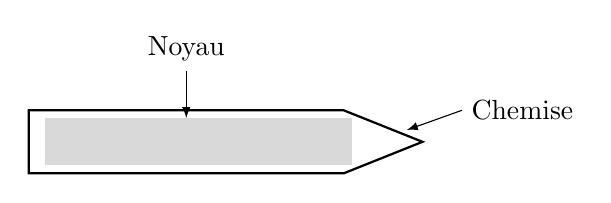
\begin{tikzpicture}[scale=1]

% Contour extérieur
\draw[thick]
(0,0)
-- (0,0.8)
-- (4,0.8)
-- (5,0.4)
-- (4,0)
-- cycle;

% Noyau
\fill[gray!30]
(0.2,0.1)
rectangle
(4.1,0.7);

% Légendes
\draw[-latex]
(2,1.3)
--
(2,0.7);

\node[above]
at (2,1.3)
{Noyau};

\draw[-latex]
(5.5,0.8)
--
(4.8,0.55);

\node[right]
at (5.5,0.8)
{Chemise};

\end{tikzpicture}

\caption{Structure simplifiée d'un projectile blindé (FMJ).}
\label{fig:fmj}

\end{figure}

\section{Contraintes des conventions internationales}

Certaines conventions internationales influencent la conception des
projectiles militaires.

Ces contraintes ont notamment favorisé l'emploi de projectiles blindés dans
de nombreuses armées.

\section{Projectile perforant}

Le projectile perforant est conçu pour améliorer la pénétration des matériaux
résistants.

Pour cela, il utilise généralement :

\begin{itemize}
    \item un noyau plus dur ;
    \item une géométrie adaptée ;
    \item une masse concentrée.
\end{itemize}

\begin{figure}[htbp]
\centering

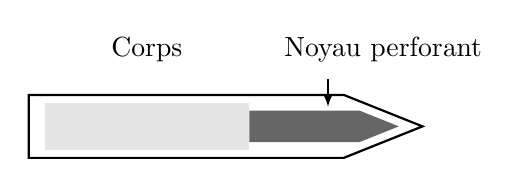
\begin{tikzpicture}[scale=1]

% Chemise
\draw[thick]
(0,0)
-- (0,0.8)
-- (4,0.8)
-- (5,0.4)
-- (4,0)
-- cycle;

% Noyau classique
\fill[gray!20]
(0.2,0.1)
rectangle
(2.8,0.7);

% Noyau perforant
\fill[black!60]
(2.8,0.2)
--
(4.2,0.2)
--
(4.7,0.4)
--
(4.2,0.6)
--
(2.8,0.6)
--
cycle;

\node[above]
at (1.5,1.1)
{Corps};

\node[above]
at (4.5,1.1)
{Noyau perforant};

\draw[-latex]
(3.8,1.0)
--
(3.8,0.65);

\end{tikzpicture}

\caption{Exemple simplifié de projectile perforant.}
\label{fig:perforant}

\end{figure}

\section{Noyaux perforants}

Les noyaux perforants peuvent être réalisés dans différents matériaux.

Les caractéristiques recherchées sont notamment :

\begin{itemize}
    \item une dureté élevée ;
    \item une bonne résistance mécanique ;
    \item une géométrie stable à l'impact.
\end{itemize}

\section{Projectile traceur}

Le projectile traceur contient une composition pyrotechnique située
généralement dans sa partie arrière.

Pendant le vol, cette composition produit une trace lumineuse visible.

\begin{figure}[htbp]
\centering

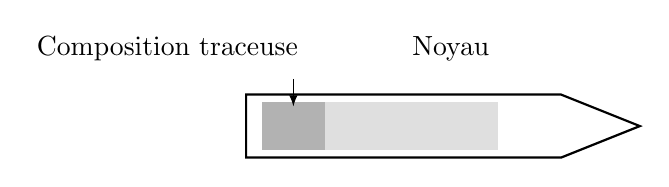
\begin{tikzpicture}[scale=1]

% Chemise
\draw[thick]
(0,0)
-- (0,0.8)
-- (4,0.8)
-- (5,0.4)
-- (4,0)
-- cycle;

% Noyau
\fill[gray!25]
(0.2,0.1)
rectangle
(3.2,0.7);

% Traceur
\fill[gray!60]
(0.2,0.1)
rectangle
(1.0,0.7);

% Légendes
\node[above]
at (2.6,1.1)
{Noyau};

\node[above]
at (-1,1.1)
{Composition traceuse};

\draw[-latex]
(0.6,1.0)
--
(0.6,0.65);

\end{tikzpicture}

\caption{Structure simplifiée d'un projectile traceur.}
\label{fig:traceur}

\end{figure}

\section{Intérêt des traceurs}

Les projectiles traceurs permettent :

\begin{itemize}
    \item de visualiser la trajectoire ;
    \item de corriger le tir ;
    \item de désigner une cible ;
    \item de faciliter certaines coordinations tactiques.
\end{itemize}

\section{Limites des traceurs}

L'utilisation de traceurs présente également certains inconvénients :

\begin{itemize}
    \item révélation de la position du tireur ;
    \item visibilité accrue du tir ;
    \item comportement balistique parfois légèrement différent.
\end{itemize}

\section{Projectile incendiaire}

Les projectiles incendiaires contiennent une composition destinée à produire
un effet thermique important après impact.

Ils sont principalement employés contre certains matériels.

\section{Projectile perforant-incendiaire}

Certaines conceptions combinent plusieurs fonctions.

Un projectile peut ainsi être à la fois :

\begin{itemize}
    \item perforant ;
    \item incendiaire.
\end{itemize}

Cette combinaison vise à améliorer l'efficacité contre certains objectifs.

\begin{figure}[htbp]
\centering

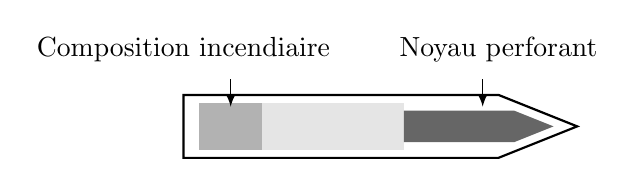
\begin{tikzpicture}[scale=1]

% Chemise
\draw[thick]
(0,0)
-- (0,0.8)
-- (4,0.8)
-- (5,0.4)
-- (4,0)
-- cycle;

% Composition incendiaire
\fill[gray!60]
(0.2,0.1)
rectangle
(1.0,0.7);

% Corps
\fill[gray!20]
(1.0,0.1)
rectangle
(2.8,0.7);

% Noyau perforant
\fill[black!60]
(2.8,0.2)
--
(4.2,0.2)
--
(4.7,0.4)
--
(4.2,0.6)
--
(2.8,0.6)
--
cycle;

\node[above]
at (0,1.1)
{Composition incendiaire};

\node[above]
at (4,1.1)
{Noyau perforant};

\draw[-latex]
(0.6,1.0)
--
(0.6,0.65);

\draw[-latex]
(3.8,1.0)
--
(3.8,0.65);

\end{tikzpicture}

\caption{Exemple simplifié de projectile perforant-incendiaire.}
\label{fig:perforant_incendiaire}

\end{figure}

\section{Projectile explosif}

Les projectiles explosifs de petit calibre restent relativement rares.

Ils sont davantage rencontrés dans les munitions de moyen et gros calibre.

\section{Projectile d'exercice}

Les armées utilisent également des projectiles destinés à l'instruction.

Leur objectif principal est de reproduire certaines caractéristiques des
munitions opérationnelles tout en réduisant les coûts.

\section{Projectile à blanc}

Les cartouches à blanc ne comportent généralement pas de projectile.

Elles permettent :

\begin{itemize}
    \item l'entraînement ;
    \item certaines cérémonies ;
    \item des simulations tactiques.
\end{itemize}

\section{Identification visuelle}

De nombreuses munitions militaires utilisent des marquages spécifiques.

Ceux-ci peuvent prendre différentes formes :

\begin{itemize}
    \item couleurs ;
    \item vernis ;
    \item marquages de pointe ;
    \item inscriptions.
\end{itemize}

\section{Normalisation}

Les systèmes d'identification varient selon :

\begin{itemize}
    \item les pays ;
    \item les époques ;
    \item les fabricants.
\end{itemize}

Aucune règle universelle ne s'applique à l'ensemble des munitions militaires.

\section{Effets recherchés}

Selon leur conception, les projectiles militaires peuvent privilégier :

\begin{itemize}
    \item la pénétration ;
    \item la visibilité ;
    \item l'effet thermique ;
    \item la précision ;
    \item la polyvalence.
\end{itemize}

\section{Vers les munitions spéciales}

Les projectiles militaires ne représentent qu'une partie de la diversité des
munitions modernes.

Le chapitre suivant abordera d'autres catégories de munitions spécialisées.

\section{À retenir}

\begin{aretenir}

\begin{itemize}
    \item Les projectiles militaires existent sous de nombreuses variantes.
    \item Les projectiles blindés sont les plus répandus.
    \item Les projectiles perforants améliorent la pénétration.
    \item Les traceurs permettent d'observer la trajectoire.
    \item Certaines conceptions combinent plusieurs fonctions.
\end{itemize}

\end{aretenir}
